%% LyX 2.3.6 created this file.  For more info, see http://www.lyx.org/.
%% Do not edit unless you really know what you are doing.
\documentclass[english,11pt,3p,number,sort&compress]{elsarticle}
\usepackage[T1]{fontenc}
\usepackage[latin9]{inputenc}
\usepackage{geometry}
\geometry{verbose,tmargin=2cm,bmargin=2cm,lmargin=2cm,rmargin=2cm,headheight=2cm,headsep=2cm,footskip=1cm}

\usepackage{color}
%\definecolor{MyRed}{rgb}{1,0,0}
\definecolor{MyRed}{rgb}{0,0,0}

\usepackage{array}
\usepackage{float}
\usepackage{bm}
\usepackage{algorithm2e}
\usepackage{amsmath}
\usepackage{amssymb}
\usepackage{stmaryrd}
\usepackage{graphicx}
\usepackage{lipsum} 

%%%%%%%%%%%%%%%%%%%%%%%%%%%%%% LyX specific LaTeX commands.
%% Because html converters don't know tabularnewline
\providecommand{\tabularnewline}{\\}

%%%%%%%%%%%%%%%%%%%%%%%%%%%%%% User specified LaTeX commands.
%\usepackage[latin1]{inputenc}

%\usepackage{amsmath}
\usepackage{natbib}
%\usepackage{subfigure}
% \usepackage{eucal}
\usepackage{dsfont}
\usepackage{comment}
\usepackage{ifthen}    
\usepackage{lscape}
\usepackage{graphicx}


\usepackage{amsmath}

\usepackage{stmaryrd} % for \llbracket and \rrbracket

\usepackage{hyperref}
\usepackage{bm}

\usepackage[subpreambles=true]{standalone}
\usepackage{xspace}
\usepackage[percent]{overpic}

%tikz stuff
\usepackage[customcolors]{hf-tikz}
\usepackage{tikz}
\usepackage{pgfplots}
\usetikzlibrary{calc,shadings,patterns,tikzmark, plotmarks, spy, 
pgfplots.polar, external, matrix, shapes.symbols,shadings,shapes, 
decorations.shapes,decorations.pathmorphing,fit,backgrounds}
\pgfplotsset{compat=1.10}   %% <-- this added

\usepgfplotslibrary{groupplots}
\usetikzlibrary{calc}
\usepackage{pgfplotstable}

\usepackage{xcolor}

% WARNING: This folder must exist
\tikzexternalize[prefix=./figs_pgfplots/tikz/]

\newcommand{\includetikz}[1]{%
	\tikzsetnextfilename{#1}%
	\input{#1}%
}

% compatibility for pgf figure
\pgfplotsset{compat=newest}

\hypersetup{urlcolor=blue, colorlinks=true}

\usepackage{amssymb}%% The amsthm package provides extended theorem environments

% Useful when sending to journals.
% Do not provide path to figures in includegraphics comand. Set them
% here instead.
\graphicspath{ {./figs/} }

% path to tikz files. Do not use path in \includetikz command
\makeatletter
\def\input@path{{./figs_pgfplots/}{./fig/}}
\makeatother

\makeatletter
\@ifundefined{showcaptionsetup}{}{%
 \PassOptionsToPackage{caption=false}{subfig}}
\usepackage{subfig}
\makeatother

\usepackage{babel}

\journal{Engineering Fracture Mechanics}

\begin{document}

\begin{frontmatter}{}

%Um primeiro título
\title{A primal hybrid-hybrid finite element method to solve tridimensional compressible, quasi-incompressible and incompressible elasticity using De Rham compatible H(div)-L2 spaces}

\author[uni]{Giovane Avancini}

\ead{giovanea@unicamp.br}

\author[uni]{Nathan Shauer}

\ead{shauer@unicamp.br}

\author[uni]{Hugo Luiz Oliveira}

\ead{hluiz@unicamp.br}

\author[uni]{Philippe R. B. Devloo}

\ead{phil@unicamp.br}

\address[uni]{Universidade Estadual de Campinas, R. Josiah Willard Gibbs 85 - Cidade Universitaria, Campinas SP, Brazil, CEP 13083-839}

%Definir se vamosar usar double-hybrid ou hybrid-hybrid. Adotei a segunda opção por enquanto
\begin{abstract}
	This work is devoted to the development of a novel primal hybrid-hybrid finite element formulation for the solution of tridimensional compressible, quasi-incompressible and incompressible elasticity problems. Hybrid-mixed methods are typically derived from an extended variational principle, where the requirement for the interlement continuity of the functions spaces is relaxed and weakly imposed using Lagrange multipliers over the element interfaces. In this sense, we propose the usage of a De Rham compatible pair H(div)-L2 for displacements and pressure, respectively. H(div) spaces naturally guarantees the continuity of the normal displacement across elements, so the tangential component conformity can be retrieved at the expense of introducing a shear stress approximation on the element edges. This leads to a semi-hybrid approach with two Lagrange multipliers so solving a saddle-point problem is inevitably even in the compreesible regime. To overcome this drawback, the shear stress can be further hybridized a second time and statically condensed to recover a positive-definite block matrix that depends on the primal variable components. In fact, there is still the need of solving a saddle point system when the bulk modulus tends to infinity, however, results have shown that this approach presents a superior stability compared to the semi-hybrid formulation. The stability, consistency and local conservation features are discussed in details. The formulation is tested and verified using 3D benchmarks for which analytical and/or numerical solutions are available, exhibiting optimal convergence rate independent of the poisson coefficient. The proposed methodology is also applied to a real-world problem, where the performance of the method is assessed in terms of accuracy and computational cost.
\end{abstract}
\begin{keyword}
\textit{Hybrid finite elements; Elasticity; H(div) approximation space; Incompressibility; Local conservation}
\end{keyword}

\end{frontmatter}{}

\section{Introduction}


According to \cite{DURAN2019}, mixed finite element formulation can \lipsum[1-2]

\section{Governing equations \label{sec:Governing-equations}}

\subsection{Strong form}

\lipsum[1-1]

\subsection{Weak form}

\lipsum[1-1]

\section{Discretization \label{sec:Discretization}}

\subsection{Finite element discretization using H(div) approximation spaces}

\lipsum[1-1]

\subsection{Comparison with H1-hybrid formulation}

\lipsum[1-1]

\subsection{Static condensation of the internal degrees of freedom}

\lipsum[1-1]

\section{Examples\label{sec:Examples}}

\subsection{Verification with manufactured solution \label{subsec:manufacsol}}


\subsubsection{Results}


\subsection{Cook's membrane problem\label{subsec:cook}}


\subsubsection{Results}


\subsection{Cantilever beam subjected to an end shear load \label{subsec:bishop}}

The case of a tridimensional cantilever beam under an end shear-load is considered. Its initial geometry is depicted in Figure \ref{fig:bishop-beam-geometry}, with $L=5$, $a=0.5$, $b=0.5$. The beam is assumed to be fixed at $z=0$ and subjected to a shear-force $F=1$ at $z=L$ pointing downwards in the $y$ direction, while the other faces are traction-free. The material is assumed to have a linear isotropic behaviour with a constant Young modulus $E=1$ whereas different values are used for the poisson coefficient in order to test the formulation for a wide range of compressibility.

% \begin{figure}[H]
% 	\centering
% 	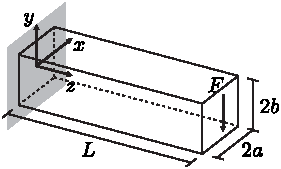
\includegraphics[width=0.5\textwidth]{bishop-beam-geometry}
% 	\caption{Cantilever beam subjected to an end shear load - geometry}
% 	\label{fig:bishop-beam-geometry}
% \end{figure}

The analytical stress state for the problem is given in \cite{bishop2014displacement} and written below:

\begin{equation} \label{eq:bishop-stress}
	\begin{aligned}
		\sigma_{xx} &= \sigma_{xy} = \sigma_{yy} = 0 \text{,}\\
		\sigma_{zz} &= \frac{F}{I} yz \text{,}\\
		\sigma_{xz} &= \frac{F}{I} \frac{2a^2}{\pi^2}\frac{\nu}{1+\nu} \sum_{n=1}^{\infty} \frac{(-1)^n}{n^2} \text{sin}\left(n\pi x/a\right) \frac{\text{sinh}\left( n\pi y/a \right)}{\text{cosh}\left( n\pi b/a \right)} \text{,}\\
		\sigma_{yz} &= \frac{F}{I} \frac{b^2-y^2}{2} + \frac{F}{I}\frac{\nu}{1+\nu} \left[ \frac{3x^2-a^2}{6} - \frac{2a^2}{\pi^2} \sum_{n=1}^{\infty} \frac{(-1)^n}{n^2} \text{cos}\left(n\pi x/a\right) \frac{\text{cosh}\left( n\pi y/a \right)}{\text{cosh}\left( n\pi b/a \right)}  \right]\text{,}\\
	\end{aligned}
\end{equation}

\noindent where $F=\int_{-b}^{b}\int_{-a}^{a}\sigma_{yz}dxdy$ and $I=4ab^3/3$ is the second moment of area about the $x$-axis. The following displacement field is obtained by integrating Equations \eqref{eq:bishop-stress} and enforcing compatibility constrains:

\begin{equation} \label{eq:bishop-displacement}
	\begin{split}
		u_x & = -\frac{F\nu}{EI} xyz \text{,}\\
		u_y & = \frac{F}{EI} \left[ \frac{\nu}{2}\left(x^2-y^2\right)z - \frac{1}{6}z^3 \right] \text{,}\\
		u_z & = \frac{F}{EI} \left[ \frac{1}{2y}\left(\nu x^2+z^2\right)z + \frac{1}{6}\nu y^3 +(1+\nu) \left(b^2 y -\frac{1}{3}y^3\right) -\frac{1}{3}a^2 \nu y \right. \\
		&\qquad\quad \left.-\frac{4a^3\nu}{\pi^3} \sum_{n=1}^{\infty} \frac{(-1)^n}{n^3} \text{cos}\left(n\pi x/a\right) \frac{\text{sinh}\left( n\pi y/a \right)}{\text{cosh}\left( n\pi b/a \right)} \right] \text{.}
	\end{split}
\end{equation}

For the analyses that follow, we kept the number of terms in the series above bounded to $n=5$. The exact solution evaluated on the boundaries of the beam is used to define the boundary conditions for the numerical analysis. At $z=0$, the exact normal and tangential displacements computed according to Eq. \eqref{eq:bishop-displacement} are prescribed, whereas surface tractions in accordance to Eq. \eqref{eq:bishop-stress} are applied on the other five faces.

Two types of partitions are used, one with hexahedral $\mathcal{S}$-elements and the other one with tetrahedral \textcolor{red}{$\mathcal{S}$}-elements. For both cases, the average element size is computed as $h_e=1/2^{n}$, where $n=\{0,1,2,3,4\}$. The coarsest ($h_e=1$) and finest ($h_e=0.0625$) meshes for each partition are shown in Figure \ref{fig:bishop-meshes}. The first analysis is carried out keeping $\nu=0.3$ as in the reference \cite{bishop2014displacement}, and a convergence test is performed for the displacement, pressure, stress and mass conservation L$^2$-norm errors, defined for the displacement as:

\begin{equation} \label{eq:bishop-errors}
	\left\| \mathbf{u} - \mathbf{u}^h \right\|_{L^2} \doteq \left[ \sum_{e=1}^{n} \int_{\Omega_e} \left(\mathbf{u} - \mathbf{u}^h\right)^2 d\Omega_e\right]^{1/2} \text{.}\\
\end{equation}

% \begin{figure}[H]
% 	\centering
% 	\subfloat[Hexahedral meshes. Coarsest (left) and finest (right)]{\includegraphics[width=1.0\textwidth]{bishop-hex-meshes}}\hfill
% 	\subfloat[Tetrahedral meshes. Coarsest (left) and finest (right)]{\includegraphics[width=1.0\textwidth]{bishop-tet-meshes}}
% 	\caption{Cantilever beam subjected to an end shear load - meshes used for the convergence test}
% 	\label{fig:bishop-meshes}
% \end{figure}

The convergence results for the aforementioned errors are shown in Figures \ref{fig:bishop-convergence-nu-03-hex}-\ref{fig:bishop-convergence-nu-03-tet}. The results show optimal convergence rates of $k+1$ for the displacement and $k$ for the remaining variables with both types of partitions. Figure \ref{fig:bishop-snapshot} plots the displacement, pressure, normal and shear stress distributions obtained with the finest hexahedral mesh using $k=2$ over the deformed configuration of the beam. The results are qualitatively similar to the reference solution, which is a strong indication of the accuracy of the proposed formulation.

% \begin{figure}
%     \centering
%     \subfloat[\label{fig:bishop-convergence-nu-03-a}Displacement]{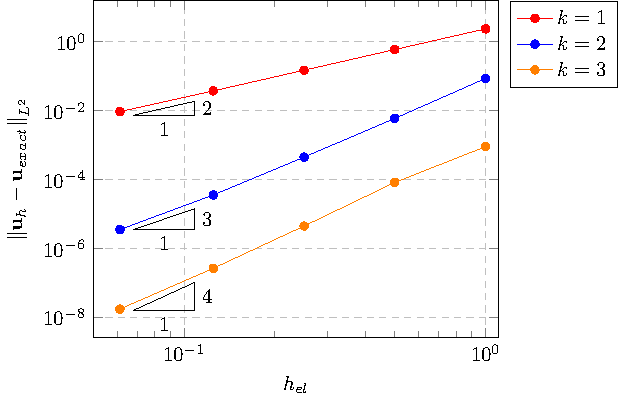
\includegraphics[trim={0cm 0cm 2.0cm 0cm},clip,scale=0.75]{Figures/bishop-disp-03.pdf}} \hfill
%     \subfloat[\label{fig:bishop-convergence-nu-03-b}Pressure]{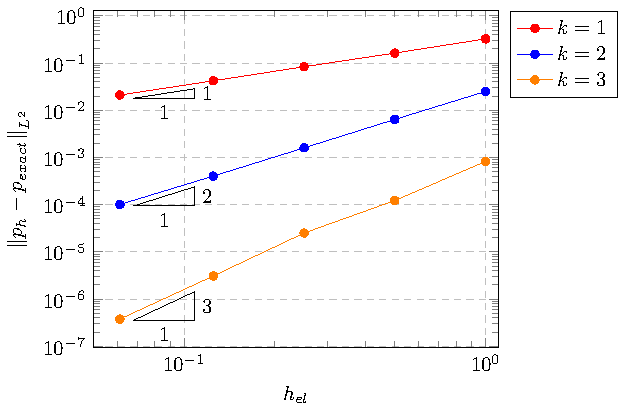
\includegraphics[trim={0cm 0cm 2.0cm 0cm},clip,scale=0.75]{Figures/bishop-pres-03.pdf}}
%     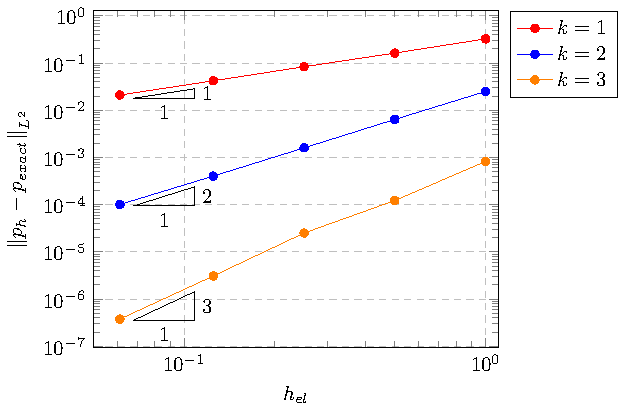
\includegraphics[trim={8.5cm 0cm 0cm 0cm},clip,scale=0.75]{Figures/bishop-pres-03.pdf}
%     \subfloat[\label{fig:bishop-convergence-nu-03-c}Stress]{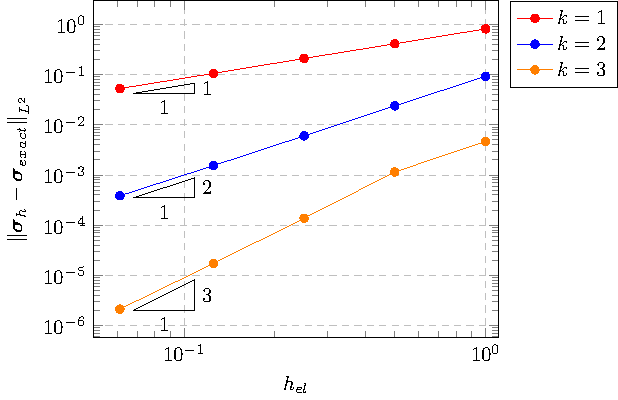
\includegraphics[trim={0cm 0cm 2.0cm 0cm},clip,scale=0.75]{Figures/bishop-stress-03.pdf}} \hfill
%     \subfloat[\label{fig:bishop-convergence-nu-03-d}Divergence]{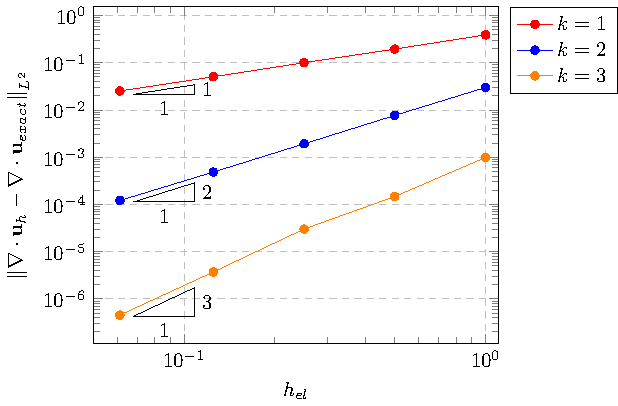
\includegraphics[trim={0cm 0cm 2.0cm 0cm},clip,scale=0.75]{Figures/bishop-div-03.pdf}}
%     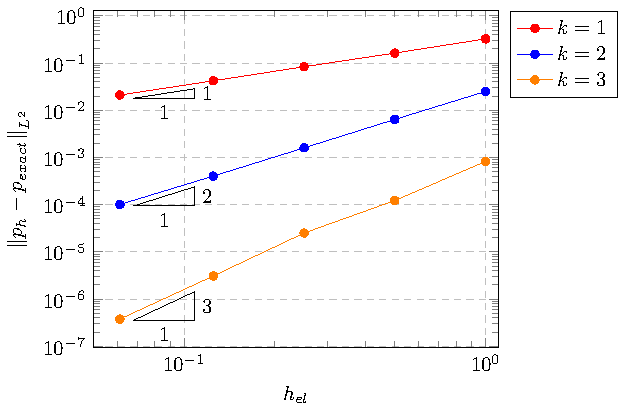
\includegraphics[trim={8.5cm 0cm 0cm 0cm},clip,scale=0.75]{Figures/bishop-pres-03.pdf}
%     \caption{Cantilever beam subjected to an end shear load - convergence analysis for the compressible case ($\nu=0.3$)}
%     \label{fig:bishop-convergence-nu-03}
% \end{figure}

% \begin{figure}
%     \centering
%     \subfloat[\label{fig:bishop-snapshot-a}Displacement]{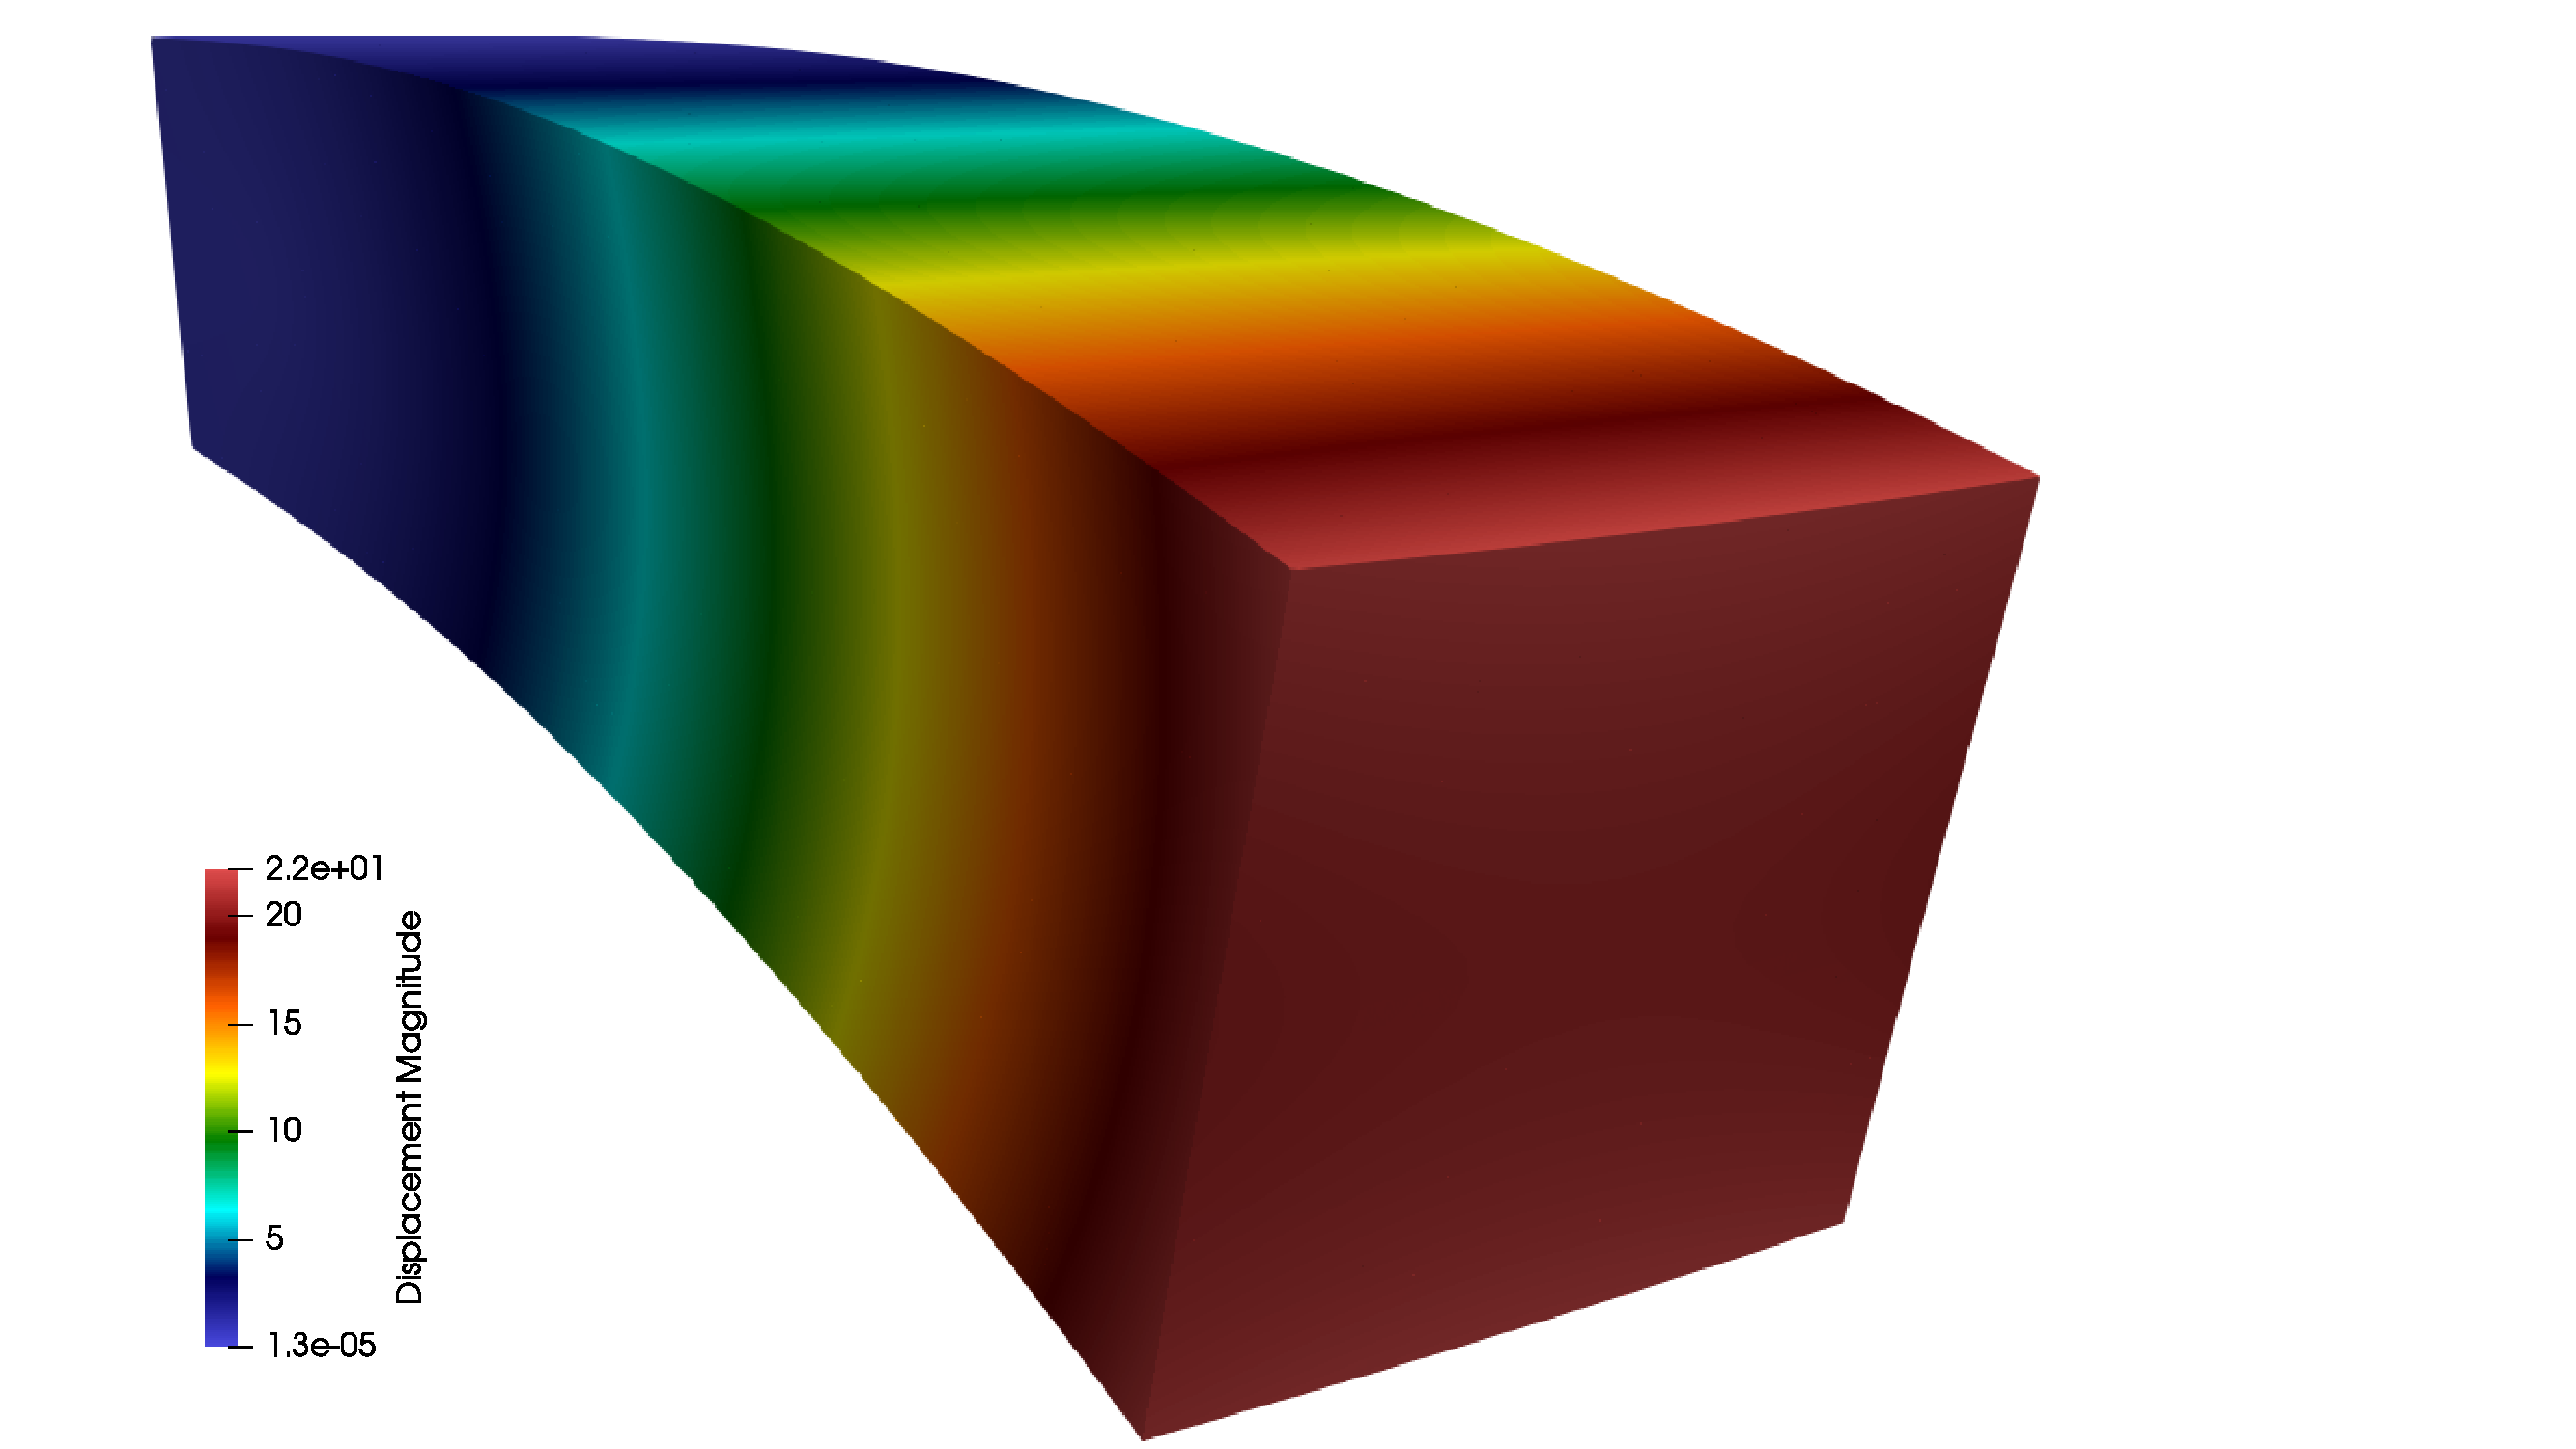
\includegraphics[trim={2.5cm 0cm 9.2cm 0cm},clip,scale=0.2]{Figures/bishop-snapshot-a.pdf}} \hfill
%     \subfloat[\label{fig:bishop-snapshot-b}Pressure]{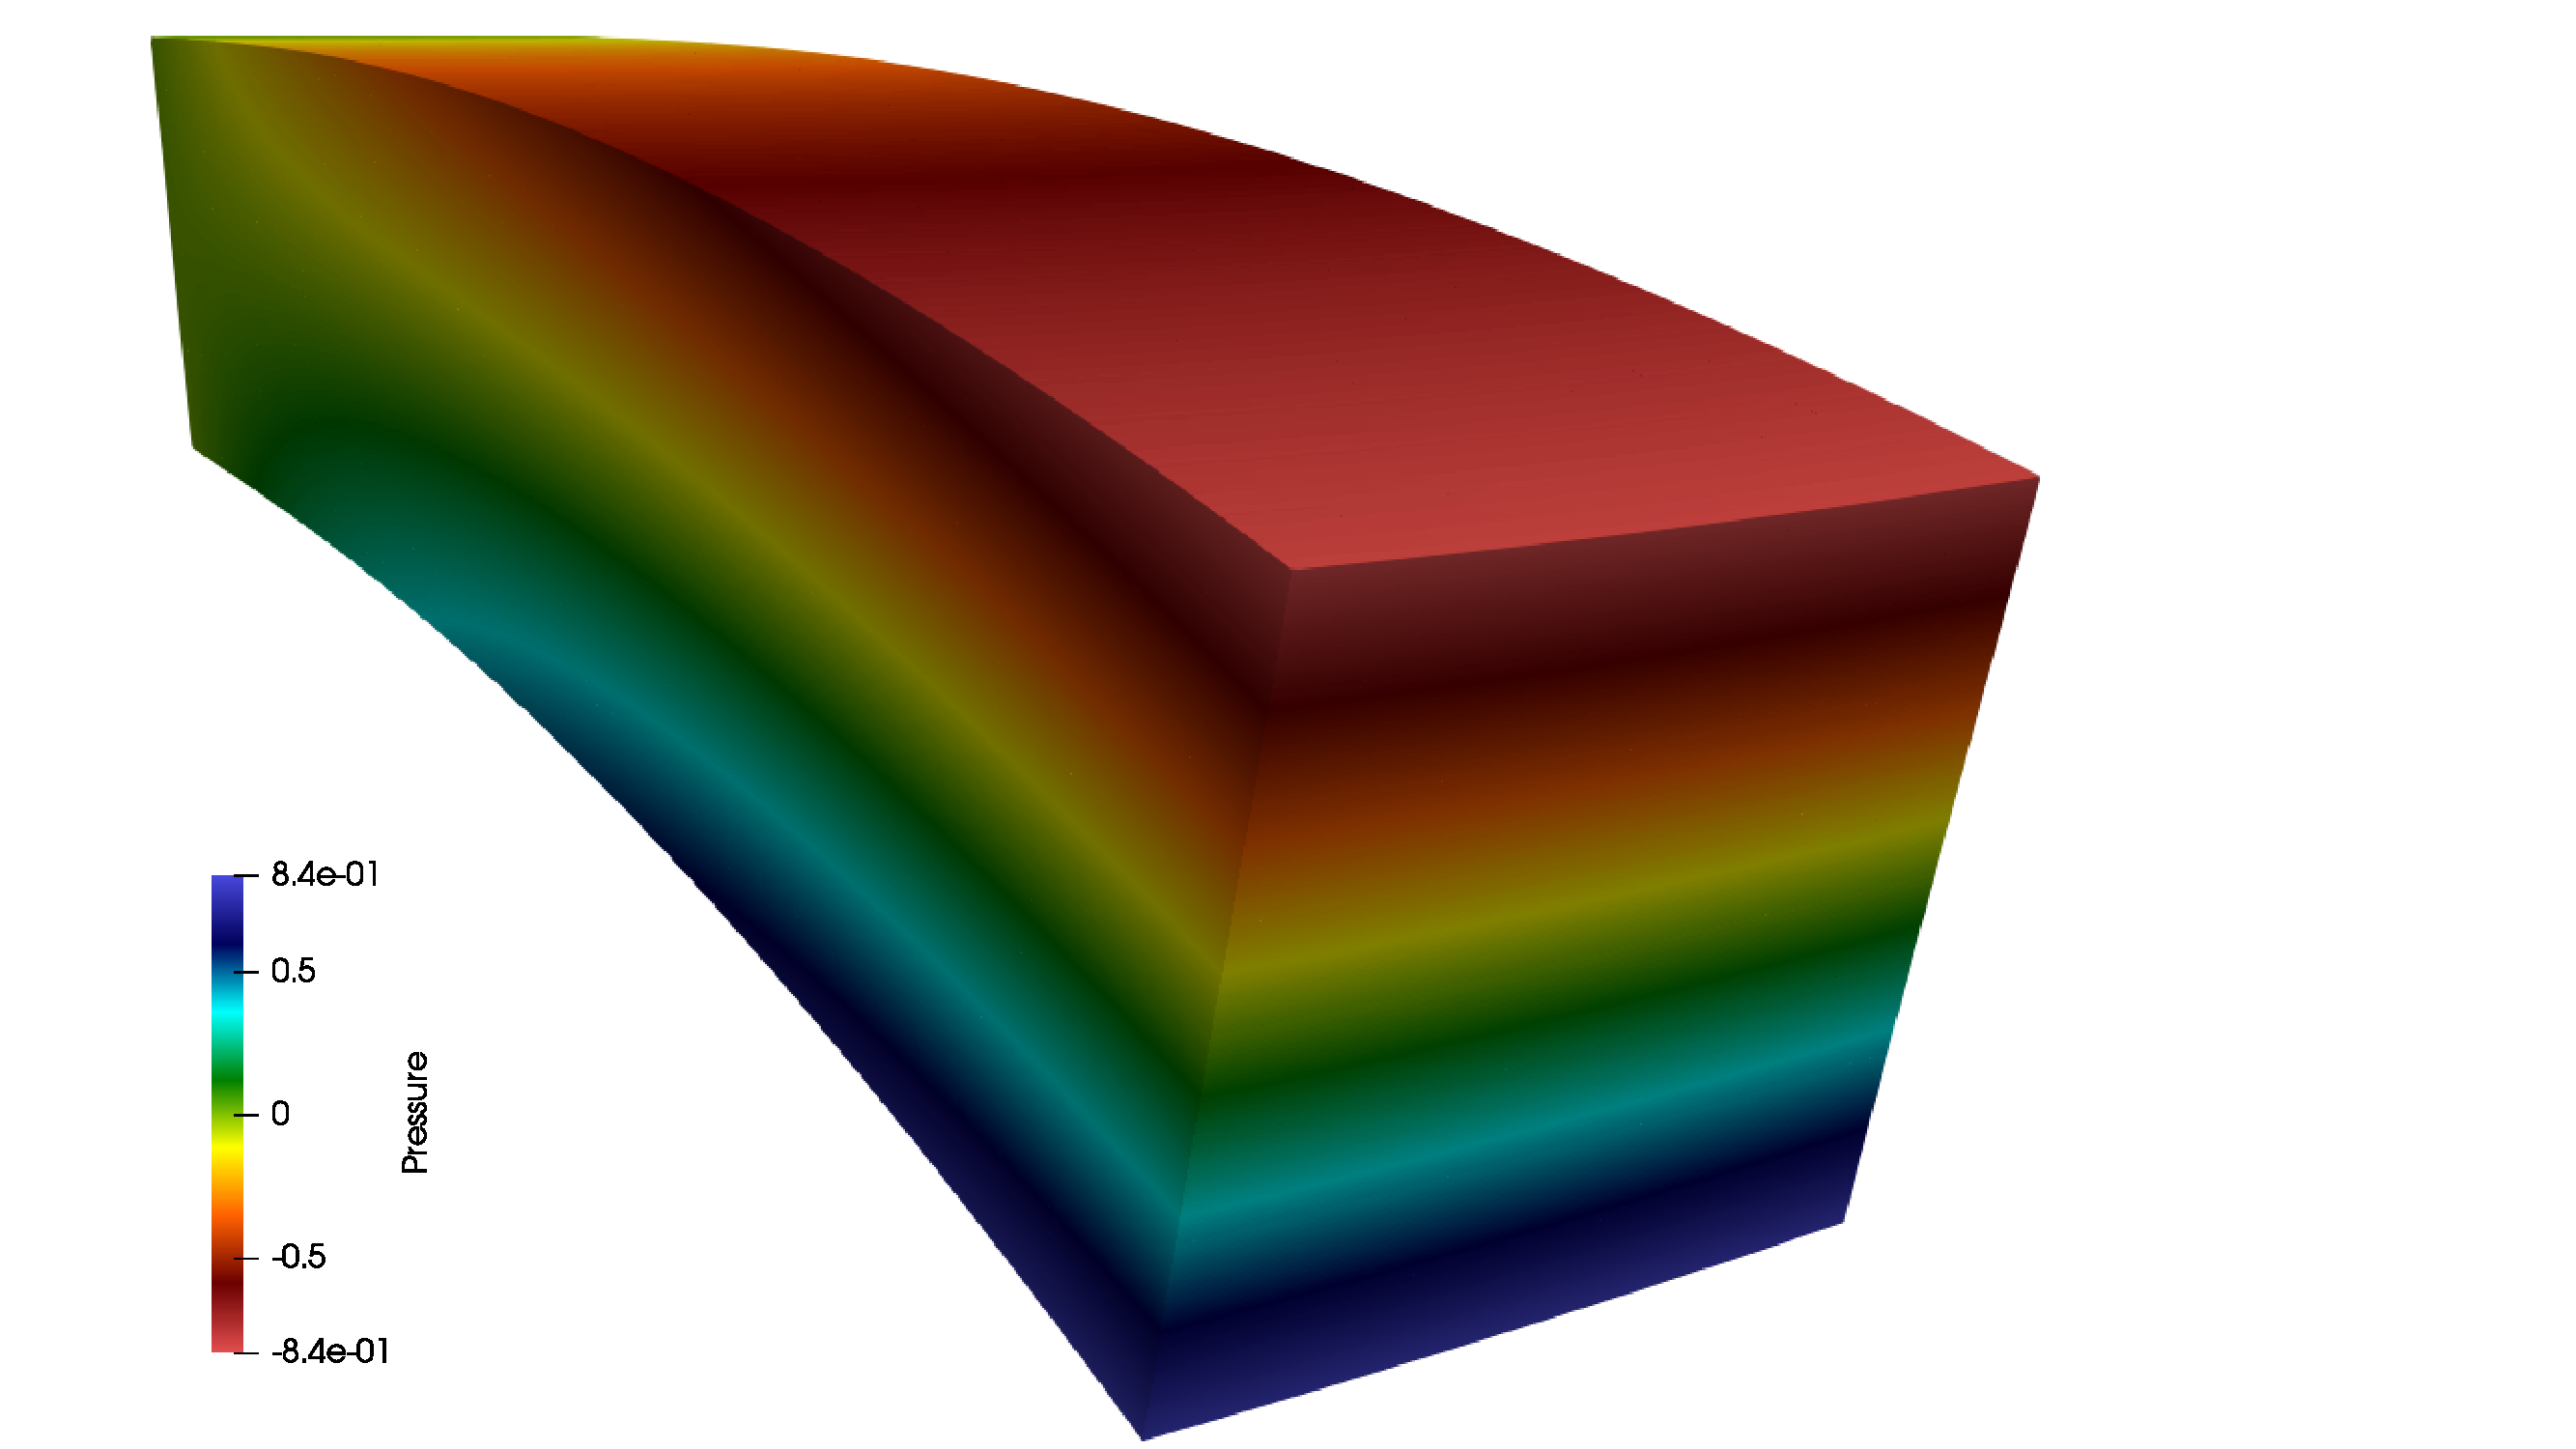
\includegraphics[trim={2.5cm 0cm 9.2cm 0cm},clip,scale=0.2]{Figures/bishop-snapshot-b.pdf}} \\
%     \subfloat[\label{fig:bishop-snapshot-c}Normal stress $\sigma_{zz}$]{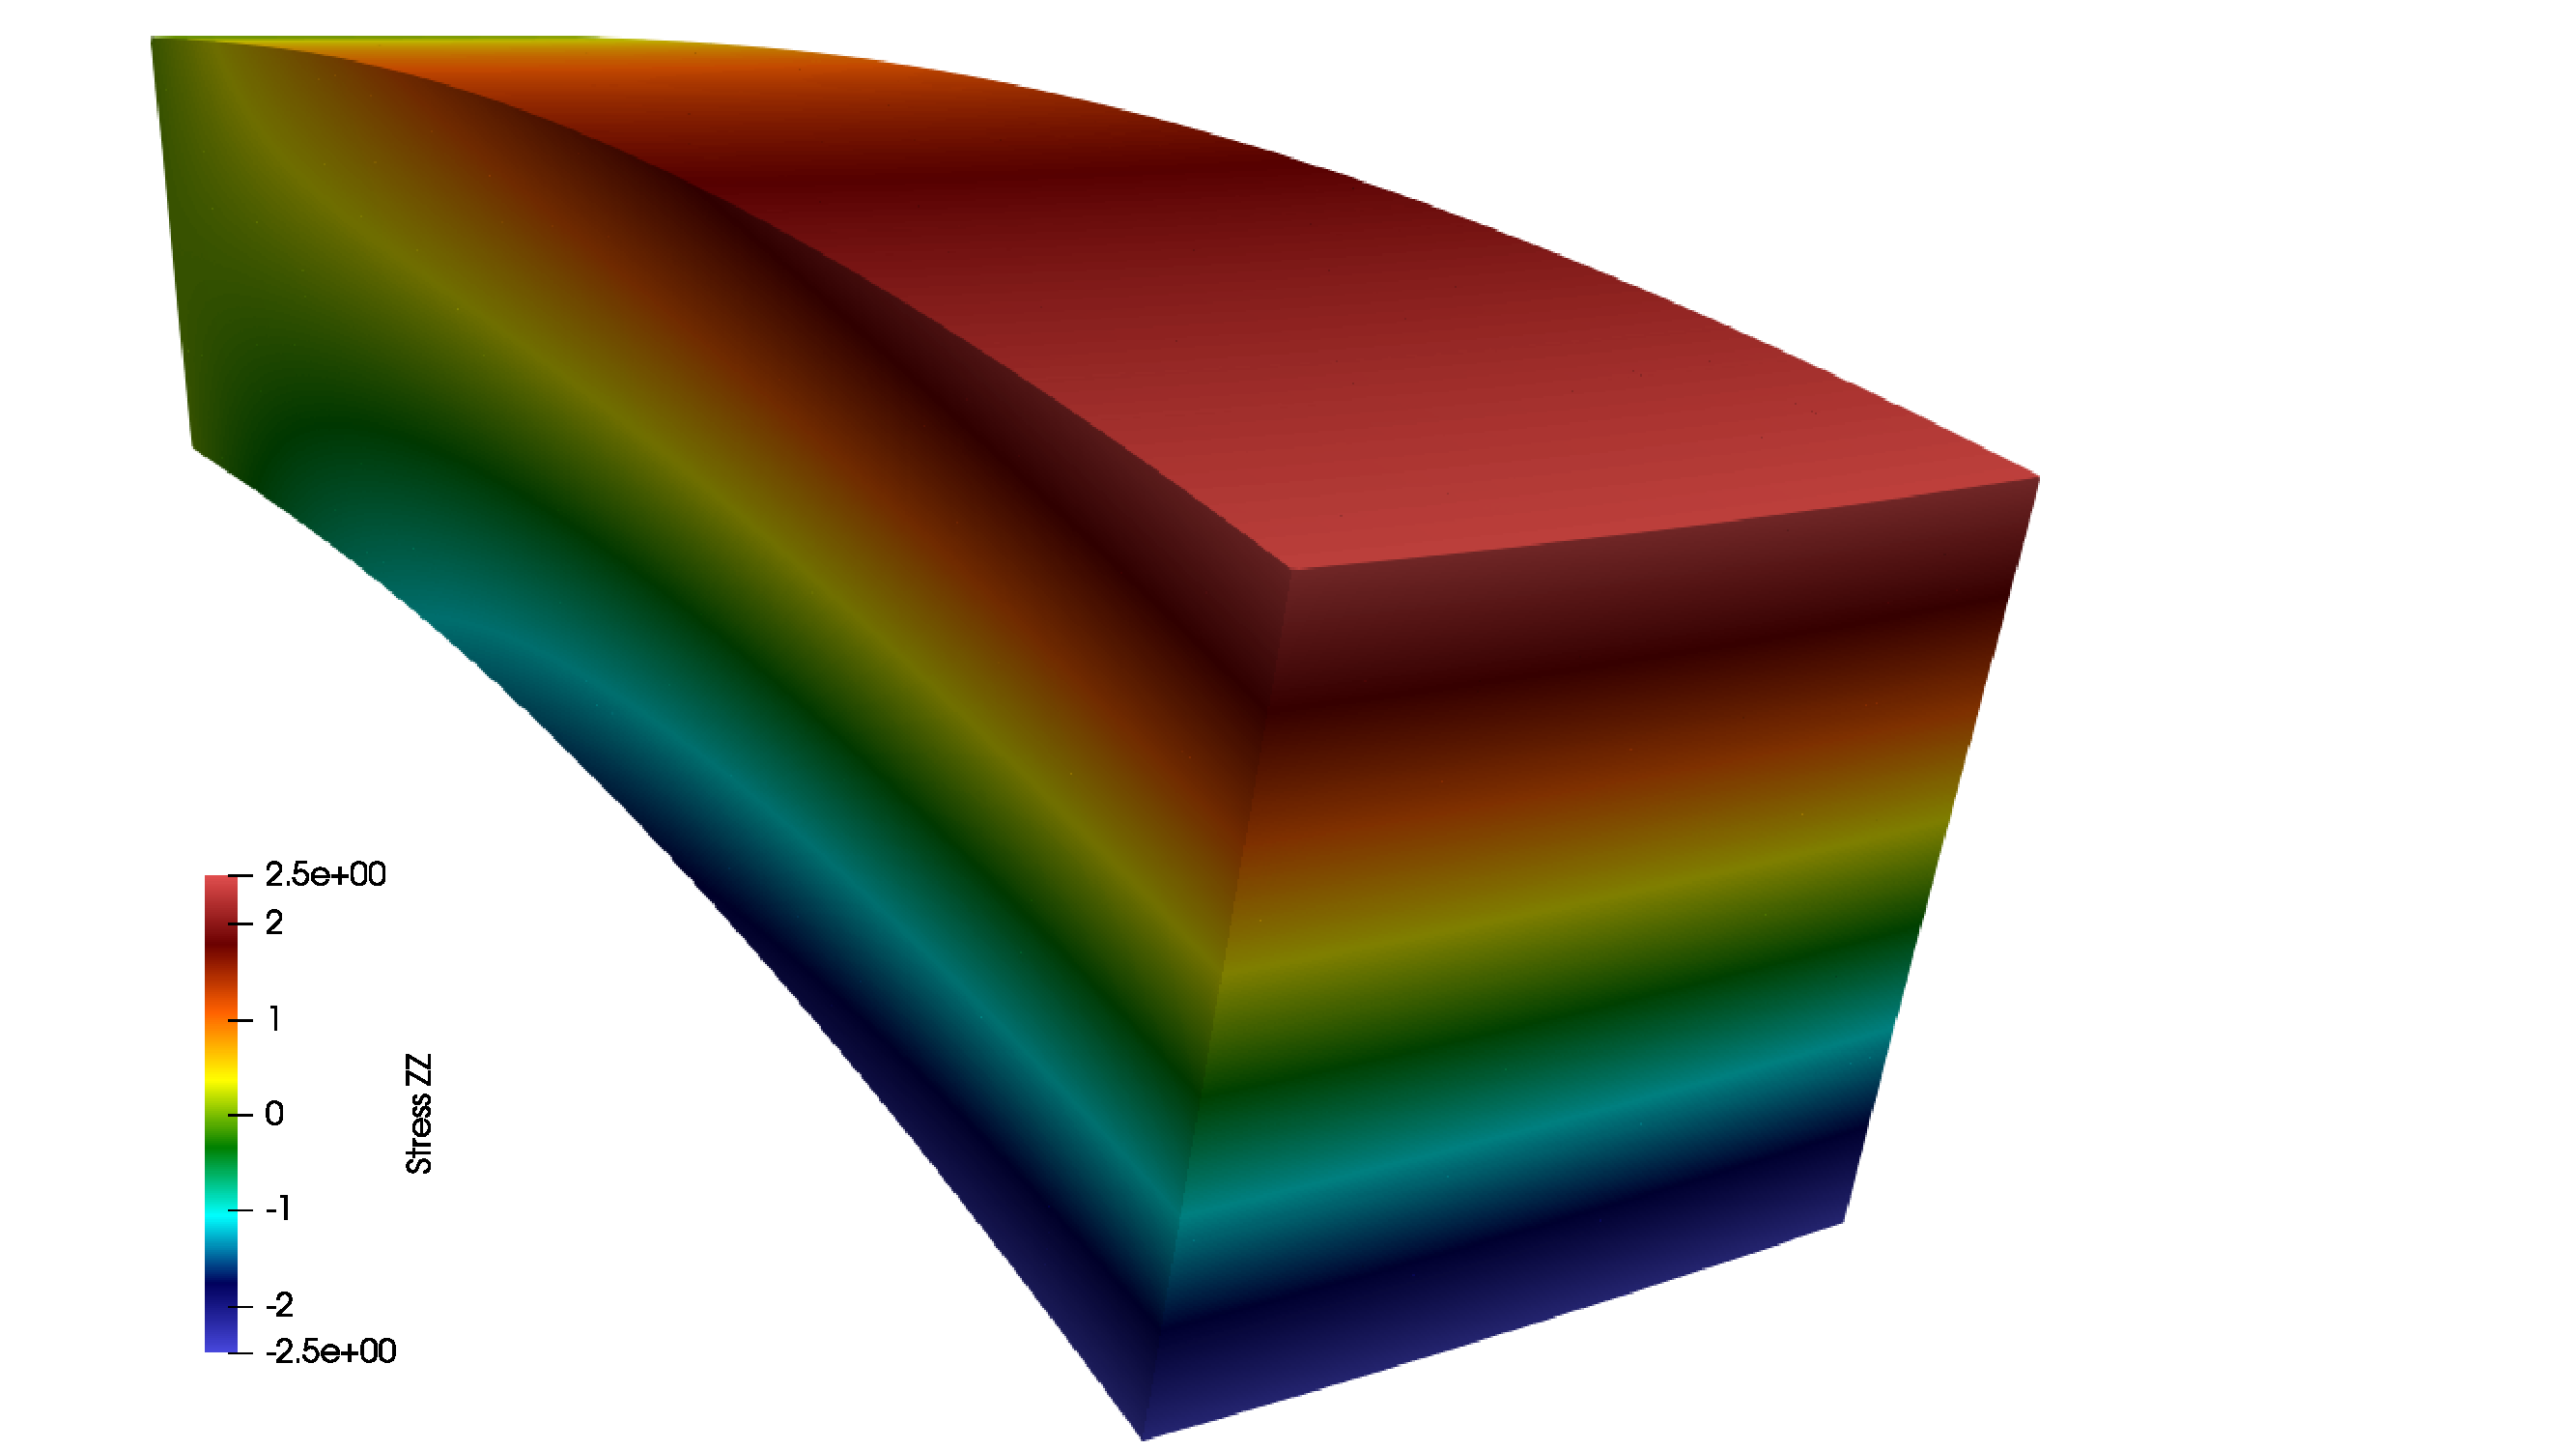
\includegraphics[trim={2.5cm 0cm 9.2cm 0cm},clip,scale=0.2]{Figures/bishop-snapshot-c.pdf}} \hfill
%     \subfloat[\label{fig:bishop-snapshot-d}Shear stress $\sigma_{yz}$]{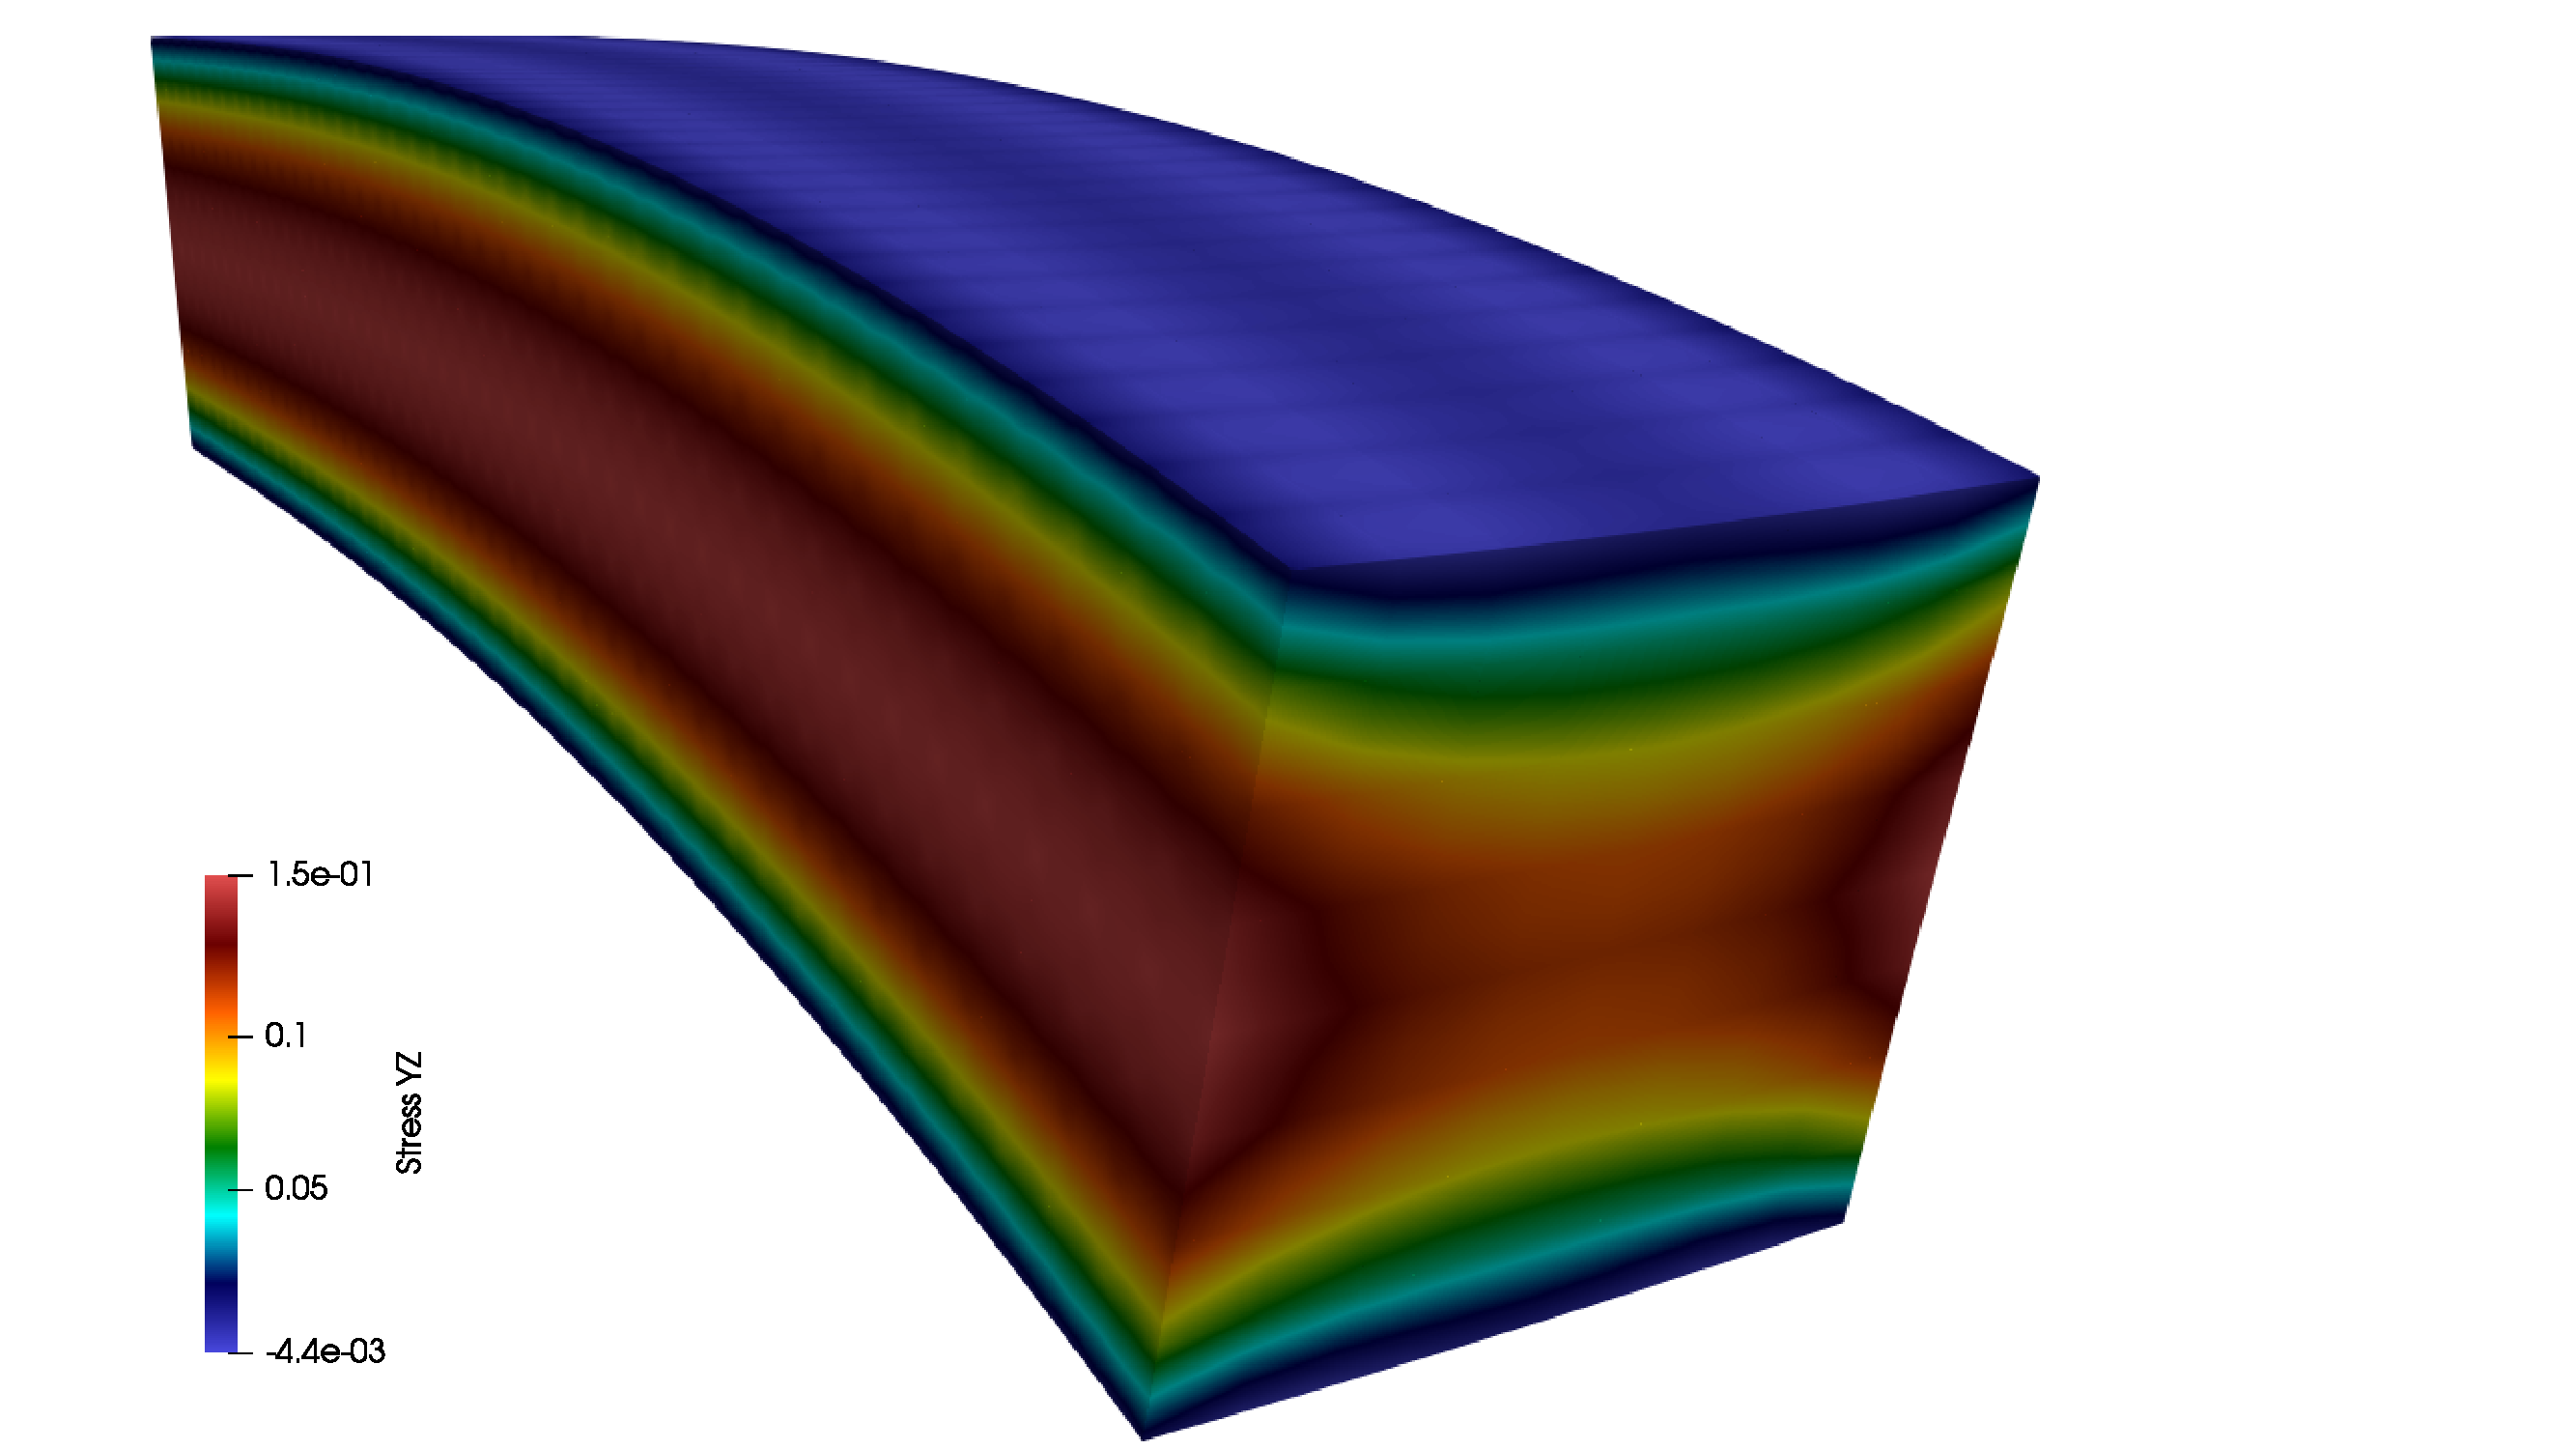
\includegraphics[trim={2.5cm 0cm 9.2cm 0cm},clip,scale=0.2]{Figures/bishop-snapshot-d.pdf}}
%     \caption{Cantilever beam subjected to an end shear load - snapshots for $\nu=0.3$}
%     \label{fig:bishop-snapshot}
% \end{figure}

In order to assess the proposed methodology in different compressibility regimes, the same analysis is performed considering $\nu=0.49$, $\nu=0.4999$, $\nu=0.499999$ and $\nu=0.5$. The convergence results are shown in Figures \ref{fig:bishop-convergence-nu-049}-\ref{fig:bishop-convergence-nu-05}, where optimal convergence rates are achieved independently of the poisson coefficient. This is a nice feature as many formulations present a locking phenomena under quasi and full incompressibility. Also, for the incompressible case ($\nu=0.5$), a divergence free displacement field is obtained even for the coarsest mesh, with the error bounded to the machine precision.

% \begin{figure}
%     \centering
%     \subfloat[\label{fig:bishop-convergence-nu-049-a}Displacement]{\includegraphics[trim={0cm 0cm 2.0cm 0cm},clip,scale=0.75]{Figures/bishop-disp-049.pdf}} \hfill
%     \subfloat[\label{fig:bishop-convergence-nu-049-b}Pressure]{\includegraphics[trim={0cm 0cm 2.0cm 0cm},clip,scale=0.75]{Figures/bishop-pres-049.pdf}}
%     \includegraphics[trim={8.5cm 0cm 0cm 0cm},clip,scale=0.75]{Figures/bishop-pres-049.pdf}
%     \subfloat[\label{fig:bishop-convergence-nu-049-c}Stress]{\includegraphics[trim={0cm 0cm 2.0cm 0cm},clip,scale=0.75]{Figures/bishop-stress-049.pdf}} \hfill
%     \subfloat[\label{fig:bishop-convergence-nu-049-d}Divergence]{\includegraphics[trim={0cm 0cm 2.0cm 0cm},clip,scale=0.75]{Figures/bishop-div-049.pdf}}
%     \includegraphics[trim={8.5cm 0cm 0cm 0cm},clip,scale=0.75]{Figures/bishop-pres-049.pdf}
%     \caption{Cantilever beam subjected to an end shear load - convergence analysis for the compressible case ($\nu=0.49$)}
%     \label{fig:bishop-convergence-nu-049}
% \end{figure}
% \begin{figure}
%     \centering
%     \subfloat[\label{fig:bishop-convergence-nu-04999-a}Displacement]{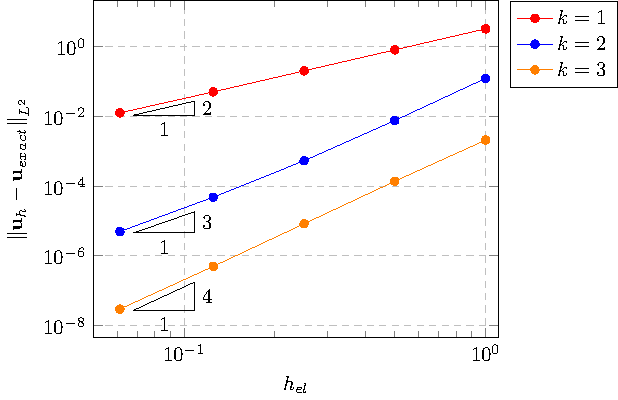
\includegraphics[trim={0cm 0cm 2.0cm 0cm},clip,scale=0.75]{Figures/bishop-disp-04999.pdf}} \hfill
%     \subfloat[\label{fig:bishop-convergence-nu-04999-b}Pressure]{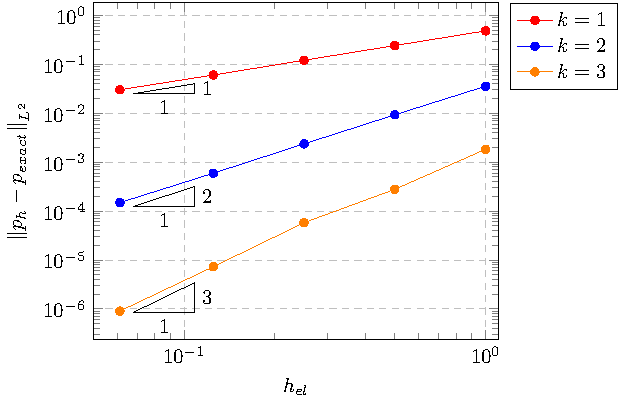
\includegraphics[trim={0cm 0cm 2.0cm 0cm},clip,scale=0.75]{Figures/bishop-pres-04999.pdf}}
%     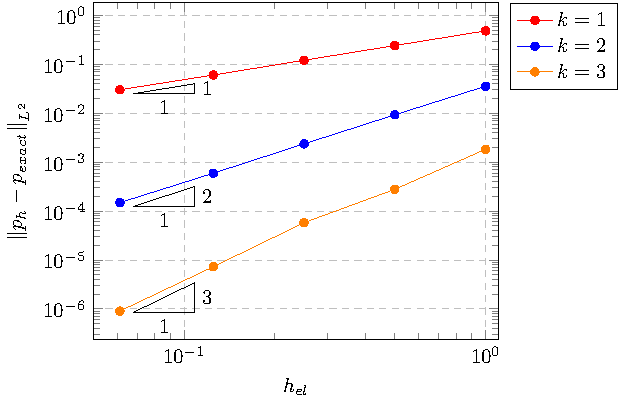
\includegraphics[trim={8.5cm 0cm 0cm 0cm},clip,scale=0.75]{Figures/bishop-pres-04999.pdf}
%     \subfloat[\label{fig:bishop-convergence-nu-04999-c}Stress]{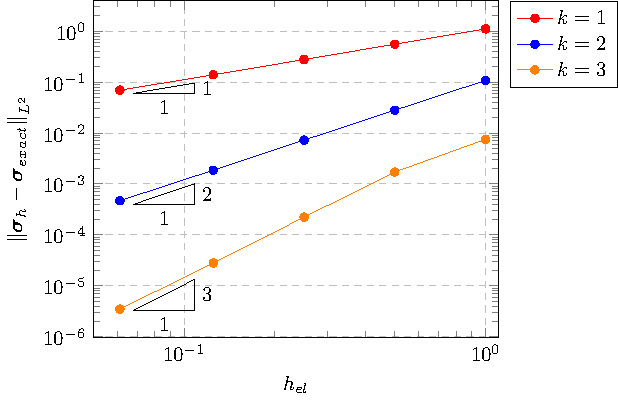
\includegraphics[trim={0cm 0cm 2.0cm 0cm},clip,scale=0.75]{Figures/bishop-stress-04999.pdf}} \hfill
%     \subfloat[\label{fig:bishop-convergence-nu-04999-d}Divergence]{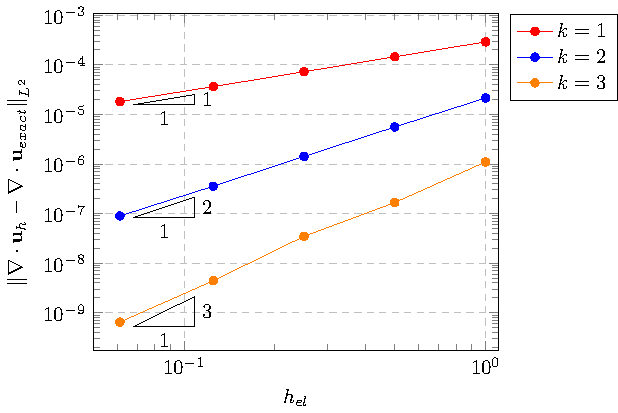
\includegraphics[trim={0cm 0cm 2.0cm 0cm},clip,scale=0.75]{Figures/bishop-div-04999.pdf}}
%     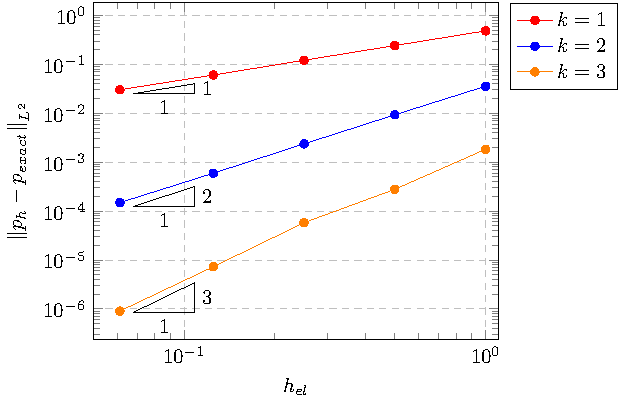
\includegraphics[trim={8.5cm 0cm 0cm 0cm},clip,scale=0.75]{Figures/bishop-pres-04999.pdf}
%     \caption{Cantilever beam subjected to an end shear load - convergence analysis for the quasi-incompressible case ($\nu=0.4999$)}
%     \label{fig:bishop-convergence-nu-04999}
% \end{figure}
% \begin{figure}
%     \centering
%     \subfloat[\label{fig:bishop-convergence-nu-0499999-a}Displacement]{\includegraphics[trim={0cm 0cm 2.0cm 0cm},clip,scale=0.75]{Figures/bishop-disp-0499999.pdf}} \hfill
%     \subfloat[\label{fig:bishop-convergence-nu-0499999-b}Pressure]{\includegraphics[trim={0cm 0cm 2.0cm 0cm},clip,scale=0.75]{Figures/bishop-pres-0499999.pdf}}
%     \includegraphics[trim={8.5cm 0cm 0cm 0cm},clip,scale=0.75]{Figures/bishop-pres-0499999.pdf}
%     \subfloat[\label{fig:bishop-convergence-nu-0499999-c}Stress]{\includegraphics[trim={0cm 0cm 2.0cm 0cm},clip,scale=0.75]{Figures/bishop-stress-0499999.pdf}} \hfill
%     \subfloat[\label{fig:bishop-convergence-nu-0499999-d}Divergence]{\includegraphics[trim={0cm 0cm 2.0cm 0cm},clip,scale=0.75]{Figures/bishop-div-0499999.pdf}}
%     \includegraphics[trim={8.5cm 0cm 0cm 0cm},clip,scale=0.75]{Figures/bishop-pres-0499999.pdf}
%     \caption{Cantilever beam subjected to an end shear load - convergence analysis for the quasi-incompressible case ($\nu=0.499999$)}
%     \label{fig:bishop-convergence-nu-0499999}
% \end{figure}
% \begin{figure}
%     \centering
%     \subfloat[\label{fig:bishop-convergence-nu-05-a}Displacement]{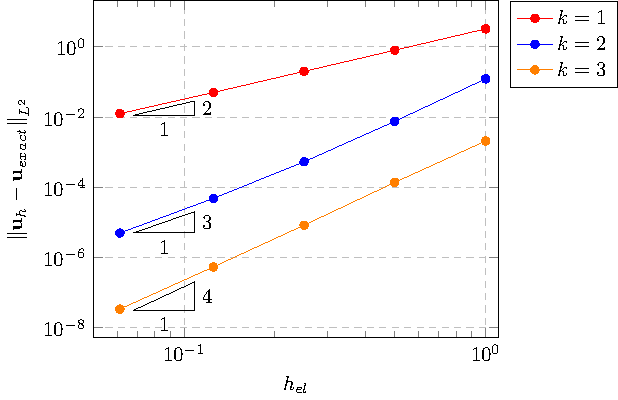
\includegraphics[trim={0cm 0cm 2.0cm 0cm},clip,scale=0.75]{Figures/bishop-disp-05.pdf}} \hfill
%     \subfloat[\label{fig:bishop-convergence-nu-05-b}Pressure]{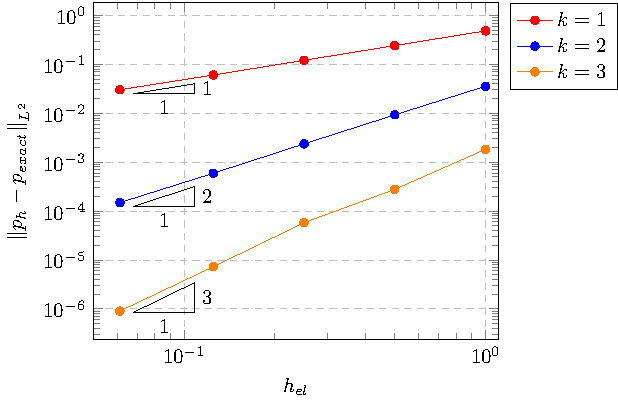
\includegraphics[trim={0cm 0cm 2.0cm 0cm},clip,scale=0.75]{Figures/bishop-pres-05.pdf}}
%     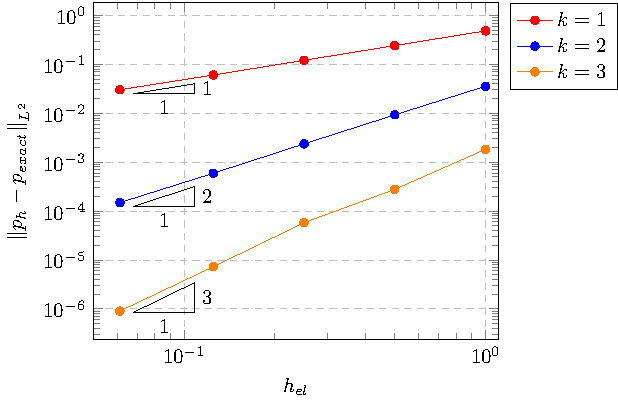
\includegraphics[trim={8.5cm 0cm 0cm 0cm},clip,scale=0.75]{Figures/bishop-pres-05.pdf}
%     \subfloat[\label{fig:bishop-convergence-nu-05-c}Stress]{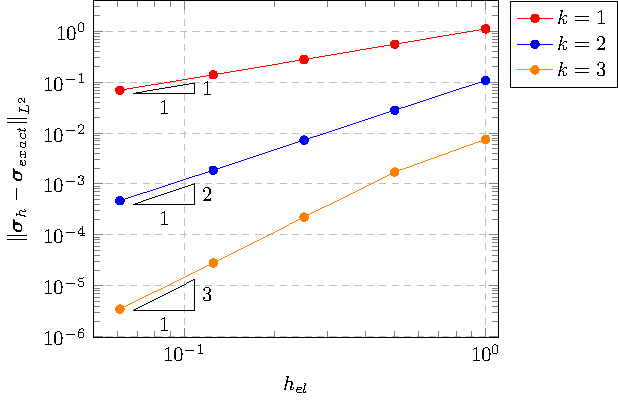
\includegraphics[trim={0cm 0cm 2.0cm 0cm},clip,scale=0.75]{Figures/bishop-stress-05.pdf}} \hfill
%     \subfloat[\label{fig:bishop-convergence-nu-05-d}Divergence]{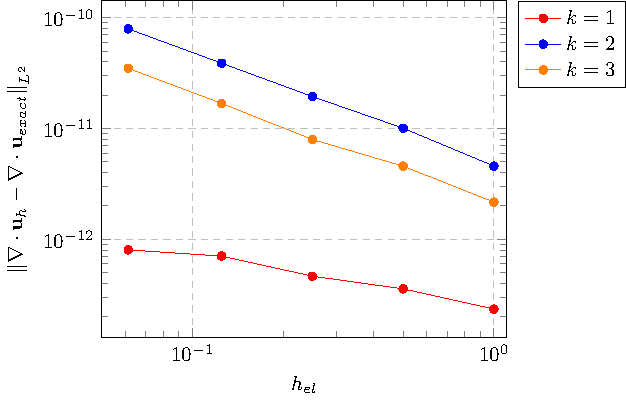
\includegraphics[trim={0cm 0cm 2.0cm 0cm},clip,scale=0.75]{Figures/bishop-div-05.pdf}}
%     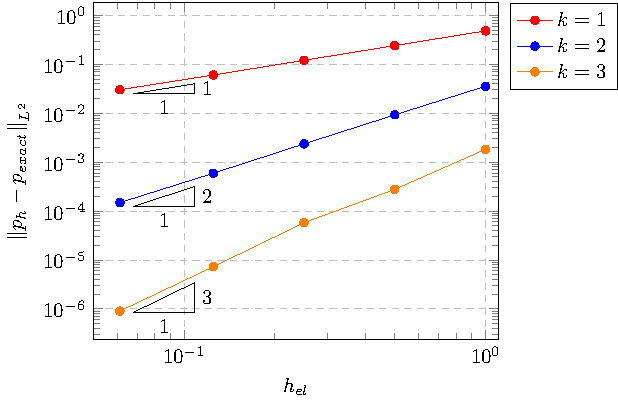
\includegraphics[trim={8.5cm 0cm 0cm 0cm},clip,scale=0.75]{Figures/bishop-pres-05.pdf}
%     \caption{Cantilever beam subjected to an end shear load - convergence analysis for the incompressible case ($\nu=0.5$)}
%     \label{fig:bishop-convergence-nu-05}
% \end{figure}

\subsection{Application problem\label{subsec:module}}


\subsubsection{Results}


\section{Conclusions}

\lipsum[1-1]

\bigskip\noindent {\bf Acknowledgments:} Authors  Nat, Gio, Hug, and Phil acknowledge the support from...

\appendix

\section{An Automatic Differentiation methodology to compute derivatives of H(div) shape functions \label{sec:Appendix-A.-Derivation}}

\lipsum[1-1]

\subsection*{The FAD package}

\lipsum[1-1]

%\bibliographystyle{plainnat}
\bibliographystyle{elsarticle-num} 
\addcontentsline{toc}{section}{\refname}
\bibliography{%
	references}

\end{document}
